\chapter{Конструкторский раздел}
В данном разделе приведено описание структуры алгоритма и отдельных его этапов с помощью диаграммы IDEF0.
Продемонстрирована схема этапа предварительной обработки текста.
Представлена архитектура и выставлены требования к пользовательскому интерфейсу разрабатываемого программного обеспечения
Продемонстрирована диаграмма классов, использующихся в работе

\section{Yake}
Общая структура метода извлечения ключевых слов представлена на рисунках \ref{fig:01a0} - \ref{fig:02a0}
\begin{figure}[!h]
	\centering
	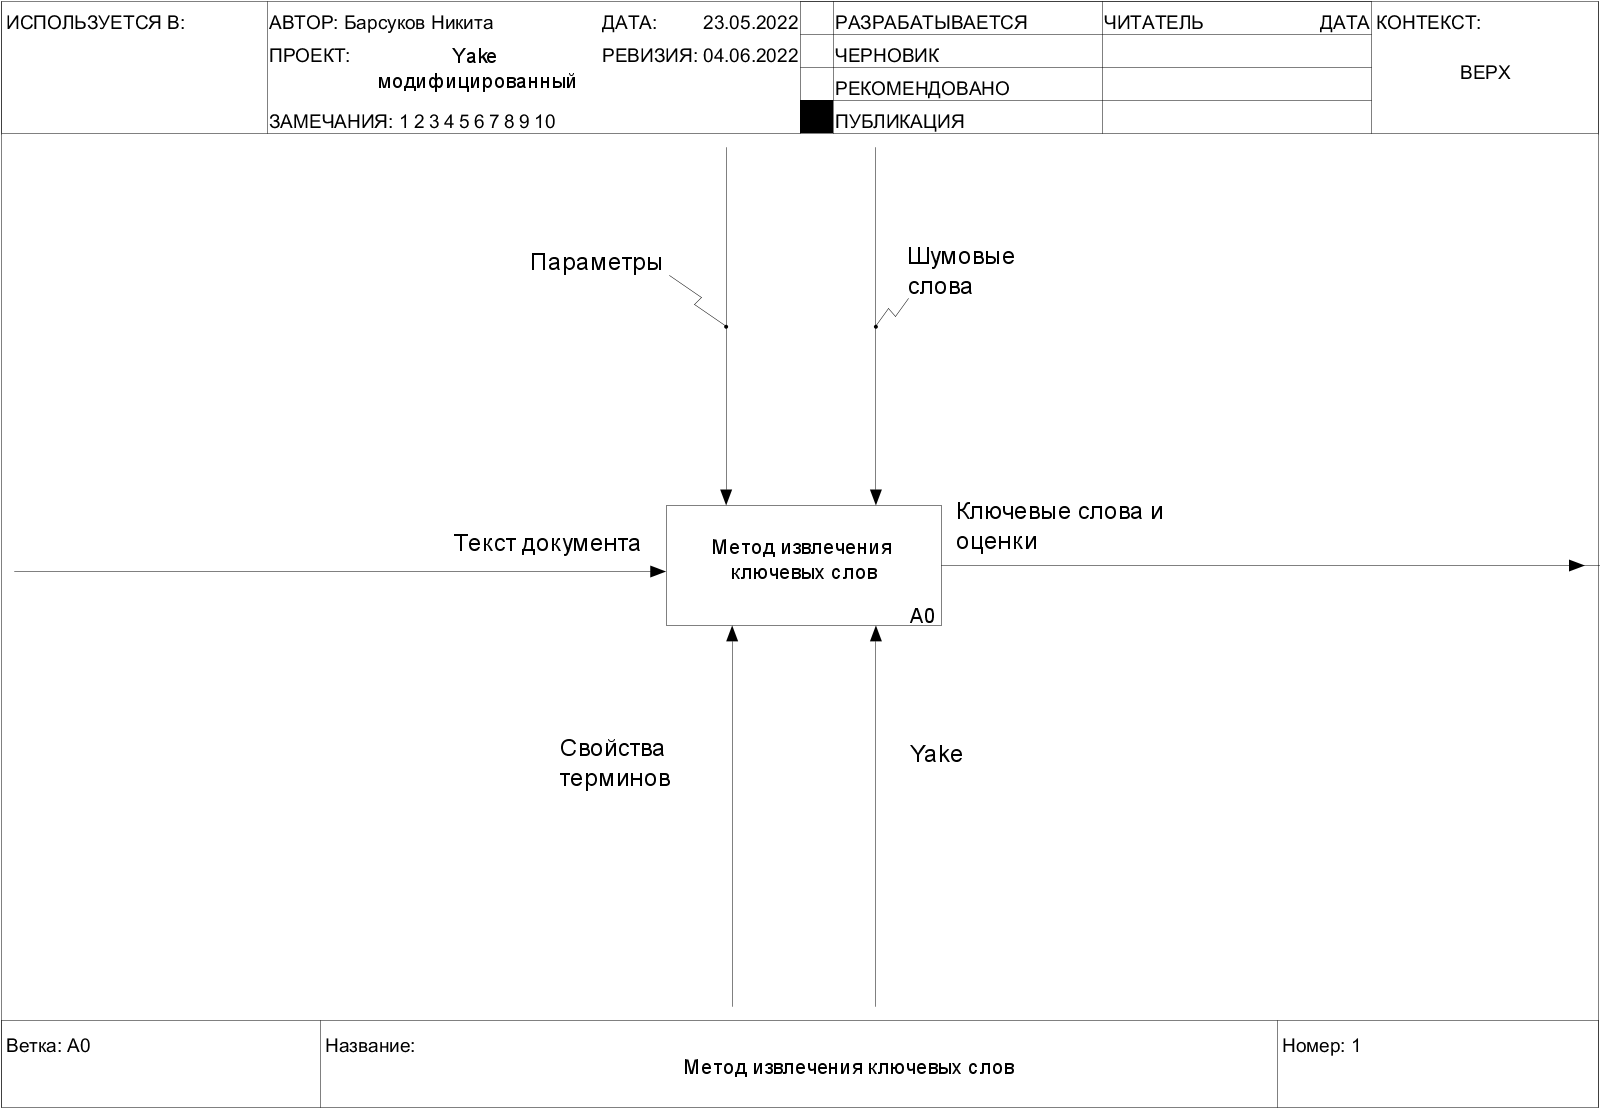
\includegraphics[width=1\linewidth]{src/img/idef0/Yake/01_A0}
	\caption{IDEF0 диаграмма разрабатываемого метода}
	\label{fig:01a0}
\end{figure}
Входными параметрами данного алгоритма являются тест извлеченный из электронного документа и язык работы.
Результатом исполнения данного метода является список, состоящий из кортежей, содержащих в себе термин и его оценку.

Данный метод можно разделить на несколько основных этапов, которые представлены на IDEF0-диаграмме, изображенной на рисунке \ref{fig:02a0}
\begin{figure}[!h]
	\centering
	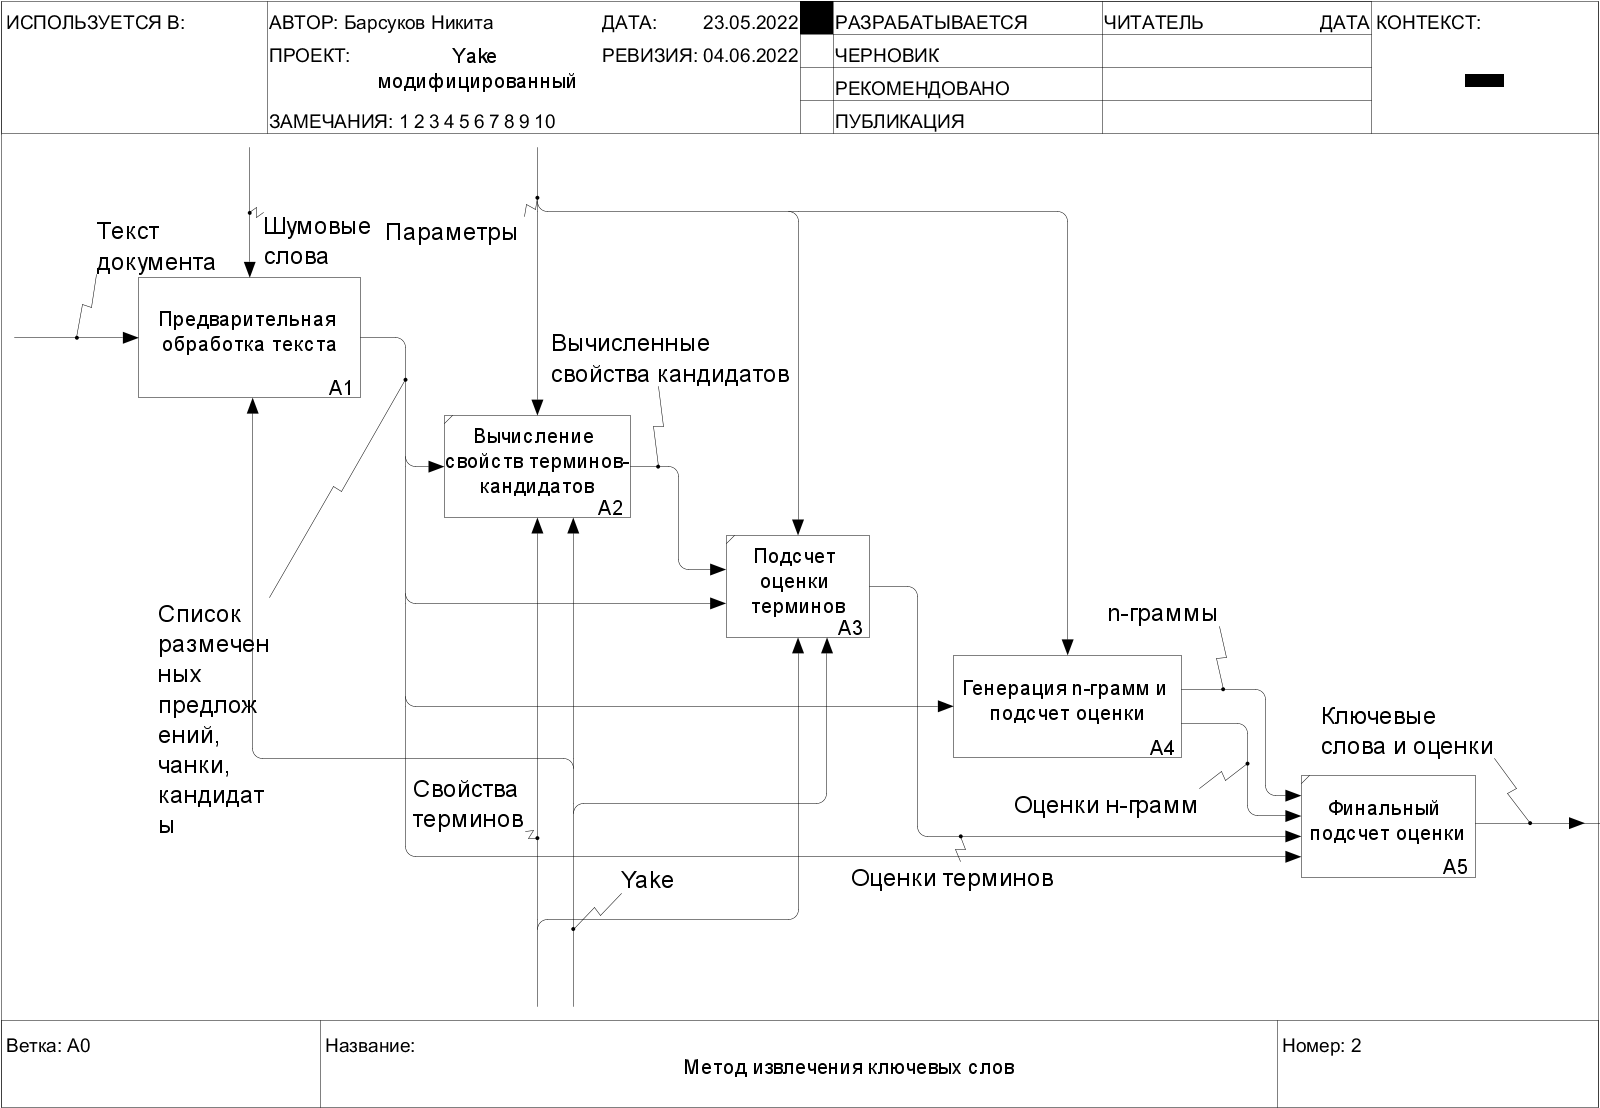
\includegraphics[width=1\linewidth]{src/img/idef0/Yake/02_A0}
	\caption{IDEF0 диаграмма модуля извлечения ключевых слов из текста}
	\label{fig:02a0}
\end{figure}

\begin{enumerate}
	\item предварительная обработка текста и выделение кандидатов (рисунок \ref{fig:02a0} блок А1)
	\item вычисление свойств термин-кандидатов (рисунок \ref{fig:02a0} блок А2)
	\item подсчет оценки кадидатов (рисунок \ref{fig:02a0} блок А3)
	\item генерация н-грамм и подсчет оценки (рисунок \ref{fig:02a0} блок А4)
	\item подсчет финальной оценки терминов (рисунок \ref{fig:02a0} блок А5)
\end{enumerate}

Формально весь процесс работы алгоритма отображен на изображениях \ref{fig:yake1} - \ref{fig:yake3}
% TODO: \usepackage{graphicx} required
\begin{figure}[!h]
	\centering
	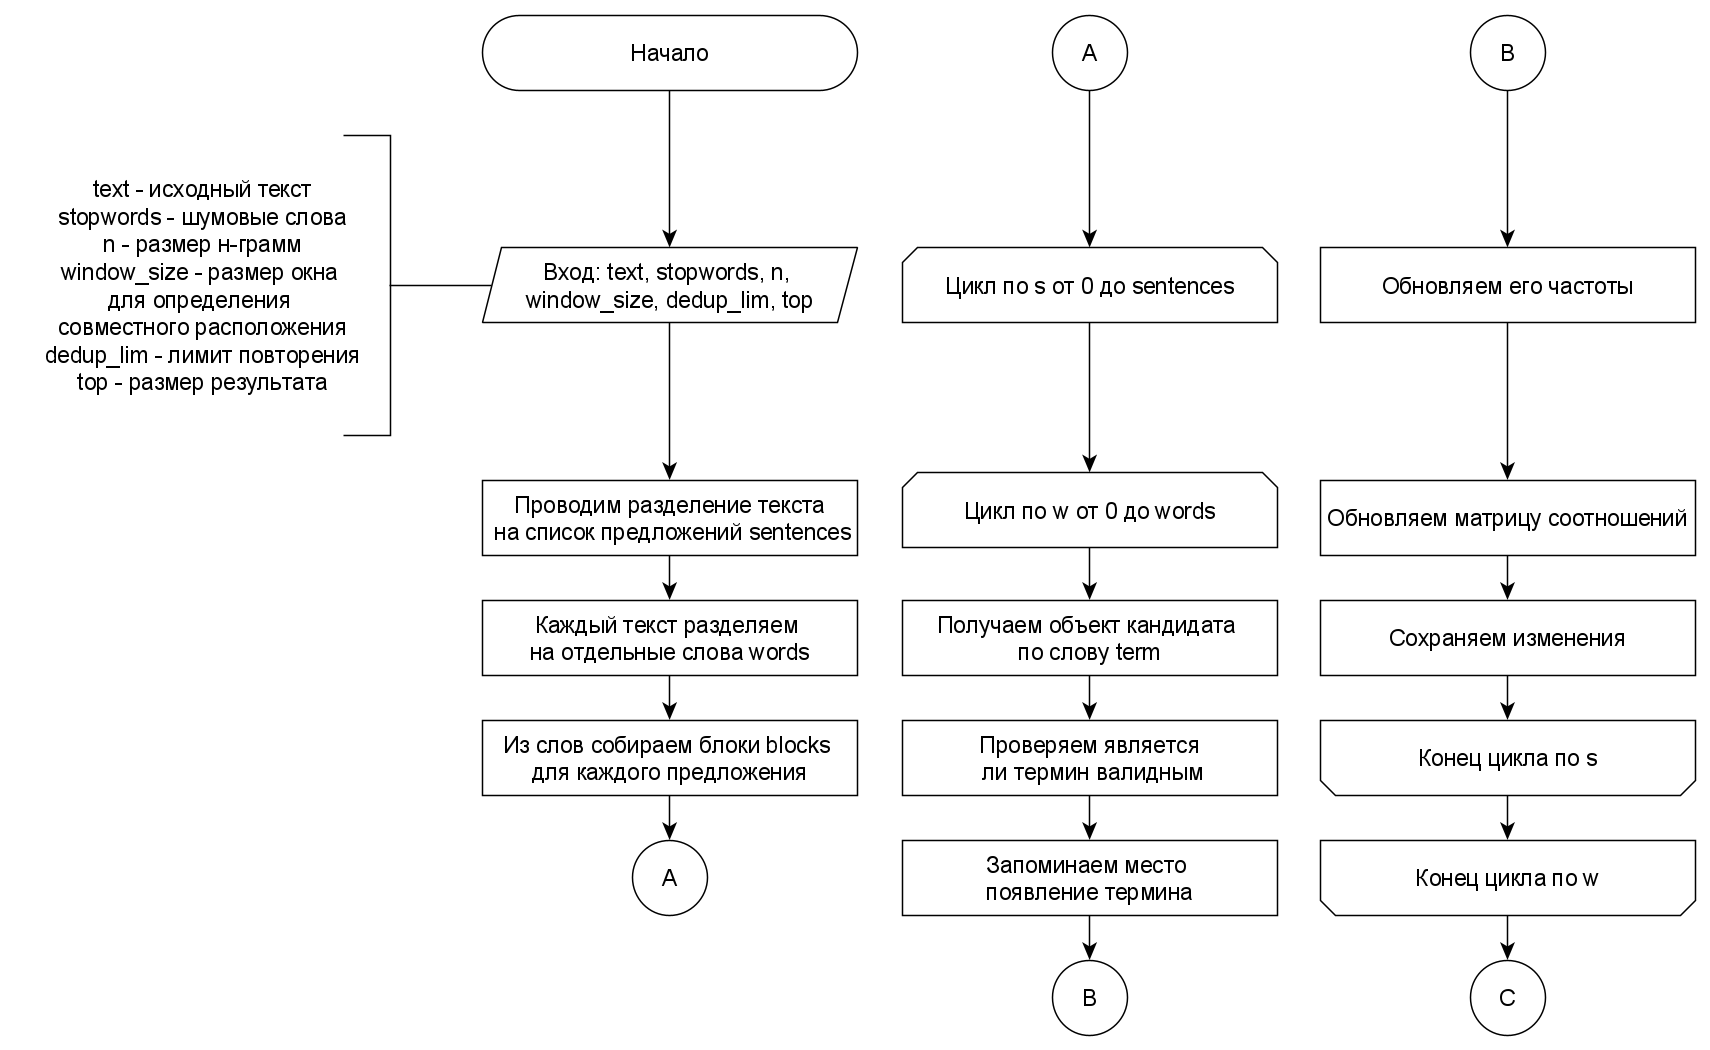
\includegraphics[width=0.7\linewidth]{src/img/design/yake_1}
	\caption{Предварительная обработка текста}
	\label{fig:yake1}
\end{figure}

% TODO: \usepackage{graphicx} required
\begin{figure}[!h]
	\centering
	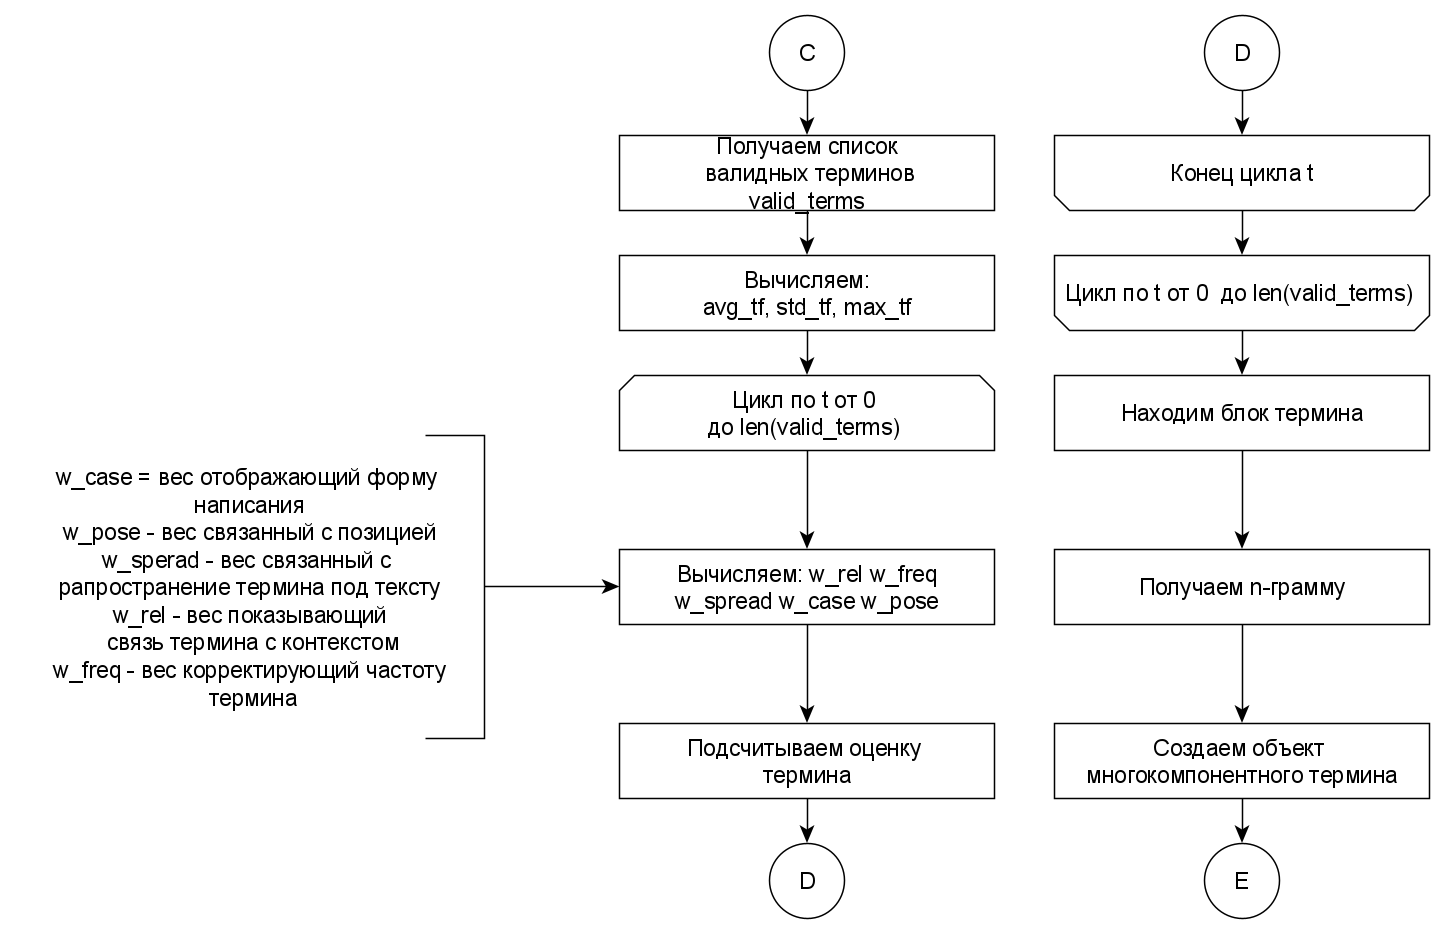
\includegraphics[width=0.7\linewidth]{src/img/design/yake_2}
	\caption{Вычисление висов методов}
	\label{fig:yake2}
\end{figure}

% TODO: \usepackage{graphicx} required
\begin{figure}[!h]
	\centering
	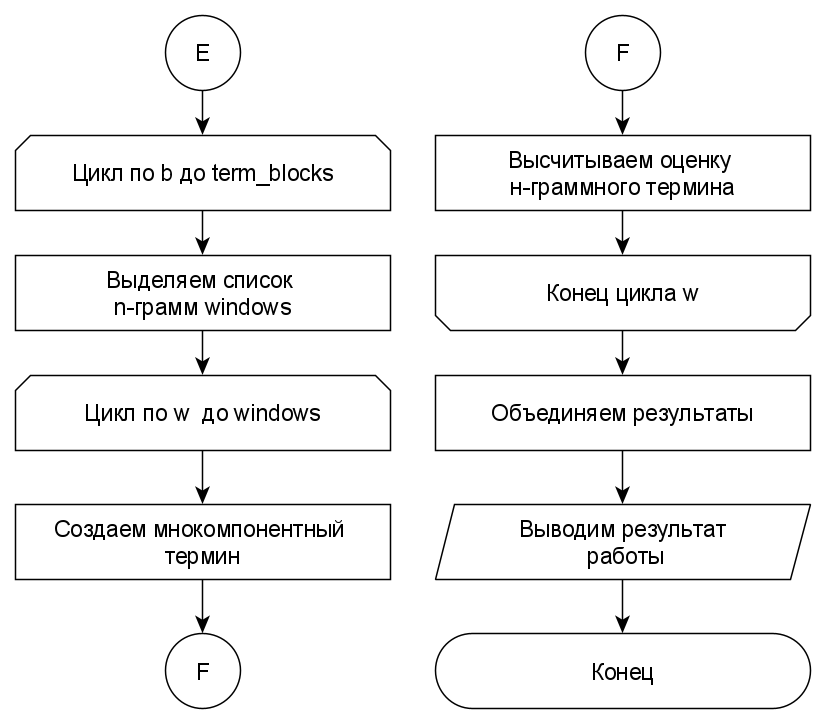
\includegraphics[width=0.7\linewidth]{src/img/design/yake_3}
	\caption{Вычисление N-грамм}
	\label{fig:yake3}
\end{figure}



В начале происходит предварительное форматирование текста, путем замены спецсимволов, таких как табуляция, перенос на новую строку и т.п. на пробелы.
Затем текст разбивается на предложения, а сами предложения на сегменты, используются на этапе оценки свойств кандидатов и построении н-грамм. 
После этого из полученных данных извлекаются уникальные термин-кандидаты с контекстной информацией.

Для оценки валидности терминов необходимо вычислить их статистические свойства и характеристики.
На рисунках \ref{fig:featureext1}, \ref{fig:featureext2} и \ref{fig:featureext3} отображена схема вычисления характеристик, где $TF$ - частота термина, $TF\_U$ - частота термина в верхнем регистре, $TF\_a$ - частота термина в виде аббревиатуры.
Теперь необходимо вычислить свойства терминов, процесс вычисления отображен на рисунках \ref{fig:calculate1}
\begin{figure}[!h]
	\centering
	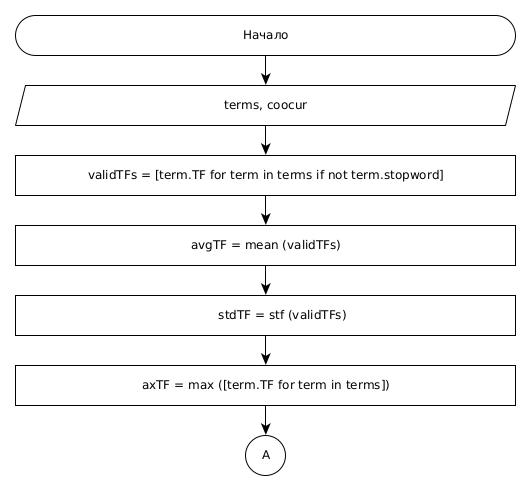
\includegraphics[width=0.7\linewidth]{src/img/design/calculate_1}
	\caption{Вычисление общих свойств}
	\label{fig:calculate1}
\end{figure}

\begin{figure}[!h]
	\centering
	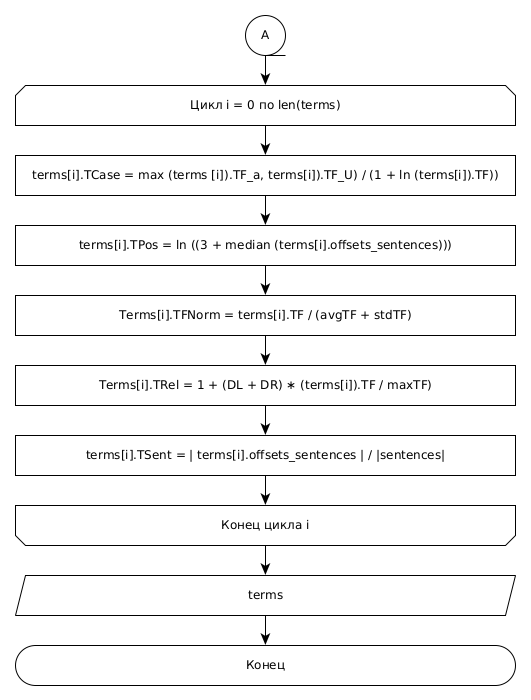
\includegraphics[width=0.7\linewidth]{src/img/design/calculate_2}
	\caption{Вычисление свойств для каждого термина}
	\label{fig:calculate2}
\end{figure}

После получениях всех свойств для каждого термина идет процесс выбора н-грамм и подсчет оценки.
Так оценка н-грамм строится на основе оценок одиночных терминов, то остается только объединить результаты и отсортировать полученный список по релевантности.


\section{Архитектура ПО}
Для реализации программного обеспечения была выбрана MVC (Model-View-Controller) архитектура, разбивающая программу на три отдельных компонента:
\begin{enumerate}
	\item представление - это отображение состояния внутренней системы;
	\item модель - это компонента, отвечающая за предоставление данных конкретным элементам системы;
	\item контроллер - это связующее звено между представлением и моделью, обрабатывает действия пользователя, полученные от представления и отдает команды модели.
\end{enumerate}
\begin{figure}[!h]
	\centering
	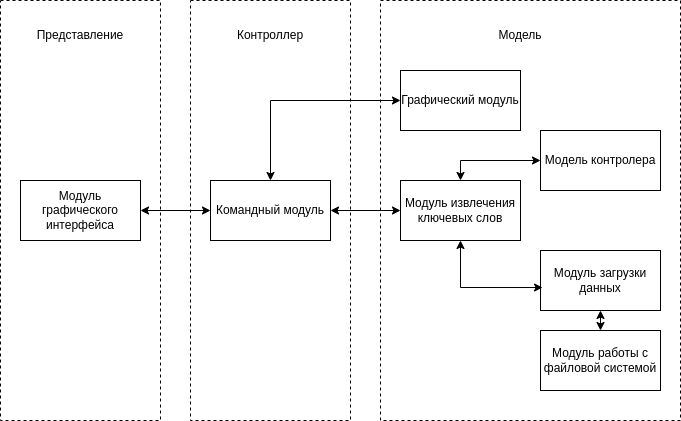
\includegraphics[width=1\linewidth]{src/img/design/mvc.drawio}
	\caption{Схематичное преставление архитектуры ПО}
	\label{fig:mvc}
\end{figure}

Благодаря использованию MVC подхода к организации архитектуры ПО, воздействие в случаи модификации или замены модуля на другие компоненты сводится к минимуму или полностью отсутствует, что добавляет системе гибкости.
Это достигается путем разделения: работы с данными, логики взаимодействия пользователя с интерфейсом.
Отличительной чертой данного решения является принцип чистой архитектуры, основанный на разделении данных.
Каждый компонент системы должен легко и просто заменяться другим и на оборот.
Это же касается используемых инструментов, библиотек, фрейворков, то есть система не привязана к конкретным технологиям и их в любой момент можно заменить.

Через графический интерфейс у пользователю должна быть возможность взаимодействия с программный ПО. 
Под взаимодействием подразумевается запуск ПО и получения результата.
Предоставляющийся функционал:
\begin{enumerate}
	\item выбор из списка методов извлечения КС от одного до нескольких алгоритмов;
	\item выбор одного или нескольких файлов через специальное окно;
	\item установка параметров для методов в отдельном окне;
	\item возможность ввести отдельно текстовую информацию.
\end{enumerate}

На рисунке \ref{fig:classdiagram} схематично отображены основные классы разрабатываемого программного продукта

Класс MainWindow - это входная точка приложения.
Он выполняет основную логику, связанную с обработкой пользовательский запросов к графическому интерфейсу.
Он взаимодействует с классом MethodControler, отвечающим за подгрузку, подготовку методов к работе и запуск процесса извлечения ключевых слов. Сами методы представлены в виде классов.

\begin{figure}[!h]
	\centering
	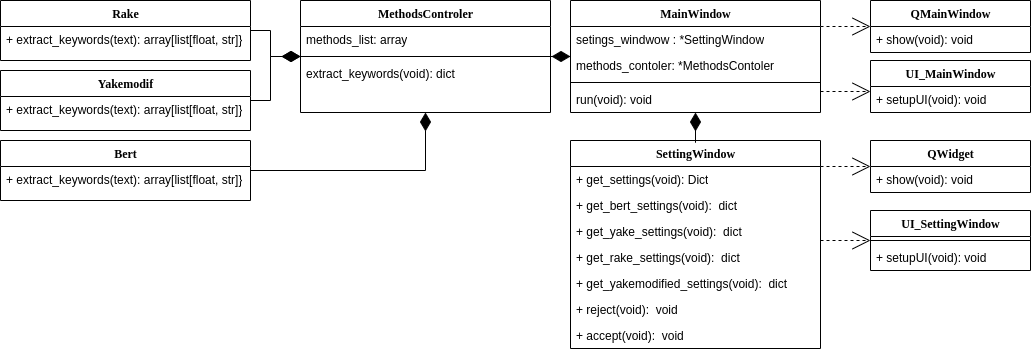
\includegraphics[width=1\linewidth]{src/img/class_diagram}
	\caption{Схематическое представление архитектуры классов программного обеспечения}
	\label{fig:classdiagram}
\end{figure}

\section{Вывод}
В данном разделе было спроектировано программное обеспечение для извлечения ключевых слов и словосочетаний из электронного документа на русском языке. 
Представлены диаграммы IDEF0 и описаны основные компоненты ПО.
Результаты проектирования:
\begin{enumerate}
	\item спроектирована архитектура разрабатываемого ПО;
	\item модификация алгоритма путем применения н-грамм;
	\item разработана структура ПО.
\end{enumerate}


